% ============================================================================
% CHAPITRE 5 — IMPLÉMENTATION DU MOTEUR DE RECOMMANDATION LinUCB (Part 1)
% ============================================================================

\section{Introduction}

Ce chapitre présente l'implémentation complète du moteur de recommandation Hybrid LinUCB du
système Guidni   un système de bandits multi-bras contextuel qui apprend en temps réel à
partir du comportement des utilisateurs. Contrairement aux systèmes de recommandation
collaboratifs classiques qui nécessitent une phase d'entraînement hors ligne sur un corpus
historique, le moteur LinUCB met à jour ses paramètres à chaque interaction utilisateur,
s'adaptant continuellement aux préférences émergentes et aux tendances saisonnières du marché
touristique de Djerba.

L'implémentation est organisée en cinq couches fonctionnelles~: le module d'ingénierie des
caractéristiques qui transforme les signaux bruts de session en vecteurs normalisés, le moteur
de scoring LinUCB qui calcule les scores d'exploitation et d'exploration, la couche de
données runtime qui gère le cache matriciel en mémoire et le traitement par lots des
événements, et enfin le tracker comportemental client couplé aux jobs de maintenance nocturne.


% ────────────────────────────────────────────────────────────────
\section{Ingénierie des caractéristiques}
% ────────────────────────────────────────────────────────────────

\subsection{vecteur utilisateur $x_{user}$}

Le constructeur du vecteur utilisateur reçoit les signaux de session courants et le profil historique pour produire un vecteur normalisé de neuf dimensions. Ce vecteur combine des signaux temporels, comportementaux et historiques dans un espace de caractéristiques unifié (valeurs entre 0 et 1).

Les quatre premières dimensions sont dédiées à un \textbf{encodage cyclique du temps} (heure et mois). Cette approche est fondamentale pour préserver la proximité temporelle : elle permet au système de comprendre que 23h et 1h du matin sont des heures proches (toutes deux nocturnes), tout comme décembre et janvier (période hivernale), ce qu'un encodage linéaire classique ne permettrait pas de capter.

Les dimensions suivantes capturent \textbf{les caractéristiques comportementales et historiques} :
\begin{itemize}
    \item \textbf{La profondeur de défilement} sur l'application.
    \item \textbf{Le temps de séjour}, lissé mathématiquement pour bien distinguer un désintérêt rapide (quelques secondes) d'une consultation prolongée, sans donner un poids démesuré aux sessions laissées ouvertes par inadvertance.
    \item \textbf{L'affinité budgétaire}, calculée à partir du prix moyen des réservations passées par rapport au plafond de la plateforme.
    \item \textbf{L'affinité maximale avec les tags}, issue du profil historique de l'utilisateur.
\end{itemize}

Enfin, la dernière dimension encode \textbf{le type de voyage} (famille, couple, solo, ou inconnu). Cette catégorisation reflète la taille du groupe social et les habitudes de consommation associées (les familles privilégiant les activités de groupe, les solos les expériences individuelles). 

Une étape finale de nettoyage au niveau du code garantit qu'aucune valeur aberrante ou non définie ne vienne corrompre les calculs matriciels en aval.


\subsection{vocabulaire de tags et le vecteur $x_{tags}$}

Le système repose sur un vocabulaire de \textbf{40 tags fixes}, 
ordonné de manière stricte et immuable. Cette immutabilité est une 
contrainte de conception fondamentale~: chaque tag occupe une position 
fixe qui détermine sa place dans les structures d'apprentissage du 
modèle. Toute modification du vocabulaire après le premier déploiement 
  même un simple réordonnancement   invaliderait l'ensemble des 
associations apprises par le système.

Pour garantir cette intégrité, une vérification automatique est 
effectuée à chaque démarrage de l'application~: si le vocabulaire a 
été altéré, le système refuse de démarrer, prévenant ainsi toute 
corruption silencieuse du modèle appris.

Chaque annonce est ensuite représentée par un \textbf{vecteur binaire} 
indiquant la présence ou l'absence de chacun des 40 tags. Ces tags 
sont issus de l'extraction automatique par LLM, avec un mécanisme de 
repli sur les tags de base de l'annonce en cas d'indisponibilité.


\subsection{produit de Kronecker $\phi$}

Le produit de Kronecker $\phi = x_{user} \otimes x_{tags}$ produit un vecteur de
360~dimensions où chaque élément $\phi[i \cdot 40 + j] = x_{user}[i] \times
x_{tags}[j]$ encode l'interaction entre la $i$\textsuperscript{e} caractéristique utilisateur
et le $j$\textsuperscript{e} tag de l'annonce.

Cette expansion capture les effets d'interaction que ni les caractéristiques utilisateur
seules ni les tags seuls ne peuvent modéliser. La dimension correspondant à
(type\_famille $\times$ tag\_pool) aura un coefficient $\theta$ élevé si les familles qui
voient des annonces piscine tendent à cliquer et réserver. La dimension
(heure\_matin $\times$ tag\_best\_evening) aura un coefficient faible ou négatif si les
utilisateurs matinaux cliquent rarement sur les activités de soirée. Ces effets d'interaction
sont la raison fondamentale du choix du modèle Hybrid LinUCB~: un modèle linéaire simple
sur la concaténation $[x_{user}; x_{tags}]$ ne capturerait que les effets marginaux, comme l'illustre le tableau~\ref{tab:phi_example}.

Une étape de validation remplace les valeurs non finies par zéro pour éviter la corruption de la matrice lors de 
la mise à jour.

\begin{table}[H]
    \centering
    \caption{Exemple de construction du vecteur $\phi$ pour un cas concret}
    \label{tab:phi_example}
    \small
    \begin{tabular}{p{2.5cm} p{11cm}}
        \toprule
        \textbf{Composant} & \textbf{Valeurs} \\
        \midrule
        Utilisateur & Famille, 10h, août, budget $\approx 300$\,TND,
                       tag\_affinity = \{pool: 0.9, beach\_access: 0.8\} \\[3pt]
        Annonce & Villa avec piscine, tags = [pool, family, luxury, wifi] \\[3pt]
        $x_{user}$ (9) & $[\sin(2\pi\cdot10/24), \cos(2\pi\cdot10/24),
                    \sin(2\pi\cdot8/12), \cos(2\pi\cdot8/12),
                    0.0, 0.0, 0.15, 0.9, 1.0]$ \\[3pt]
        $x_{tags}$ (40) & $[0,...,0, \underbrace{1.0}_{\text{family}},
                    0,..., \underbrace{1.0}_{\text{luxury}}, 0,...,
                    \underbrace{1.0}_{\text{pool}}, 0,...,
                    \underbrace{1.0}_{\text{wifi}}]$ \\[3pt]
        $\phi$ (360) & $\phi[\text{index(trip\_type)} \cdot 40 + \text{index(pool)}]
                    = 1.0 \times 1.0 = 1.0$ (forte interaction
                    famille $\times$ piscine) \\
        \bottomrule
    \end{tabular}
\end{table}


% ────────────────────────────────────────────────────────────────
\section{Moteur de scoring LinUCB}
% ────────────────────────────────────────────────────────────────

\subsection{Score UCB et paramètres}

Le score UCB combine exploitation, exploration et bonus de sous-exposition :
\[ \text{Score} = \underbrace{\hat{\theta}^\top \phi}_{\text{Exploitation}} + \underbrace{\alpha \sqrt{\max(\phi^\top A^{-1} \phi, 0)}}_{\text{Exploration}} + \underbrace{\delta_{\text{sous-exp}} \cdot 0.15}_{\text{Bonus}} \]
où $\hat{\theta}$ est estimé par résolution du système $A\hat{\theta} = b$ . 
Le paramètre $\alpha = 0.3$ est calibré pour les sessions touristiques courtes, offrant un compromis 
optimal entre pertinence immédiate et découverte rapide des nouvelles annonces. La décomposition du 
score est journalisée pour faciliter le débogage et l'analyse A/B.


\subsection{Mise à jour des matrices et récompenses}

La mise à jour en ligne suit $A \mathrel{+}= \phi \phi^\top$ et $b \mathrel{+}= r \cdot \phi$, 
équivalente à une descente de gradient avec régularisation $L_2$ (grâce à l'initialisation $A = I$). 
Les récompenses $r$ s'échelonnent de -0.2 (\textit{quick\_exit}) à 1.0 (\textit{reservation}), 
avec des valeurs intermédiaires progressant selon l'engagement (clic, interaction, favoris) et 
la durée de séjour. 

Un mécanisme de \textit{delta par session} empêche l'inflation des récompenses en évitant le 
double comptage : $\Delta r = \max(r_{new}, r_{max}) - r_{max}$. Seule la progression vers 
la récompense maximale observée est comptabilisée. Enfin, une vérification de santé assure que 
 $A$ reste définie positive. En cas d'échec numérique, le système tente d'abord un repli par 
moindres carrés (\texttt{lstsq}) pour préserver l'historique, avant de réinitialiser les 
matrices ($A = I$, $b = 0$) en dernier recours.
% ============================================================================
% CHAPITRE 5 — Part 2: Ranker, Tag Extractor, Runtime, Tracker, Jobs
% ============================================================================



\section{Extracteur de tags par LLM}

Le taggage manuel de centaines d'annonces est impraticable et source 
d'erreurs. Les approches à base de règles ne captureraient pas la 
richesse sémantique des descriptions en langage naturel~: un LLM peut 
lire une description telle que \og{}suite romantique avec vue sur mer 
et piscine privée\fg{} et la projeter sur les tags corrects du 
vocabulaire sans aucune règle explicite.

Le modèle est instruit de n'extraire que des tags appartenant 
strictement au vocabulaire fixe de la plateforme~; tout tag généré 
en dehors de ce vocabulaire est automatiquement écarté, éliminant 
le risque d'hallucination sémantique. En l'absence de tags valides, 
un tag de repli générique est assigné pour garantir qu'aucune annonce 
ne reste sans catégorisation.

Les défaillances transitoires de l'API sont gérées par un mécanisme 
de tentatives automatiques~; en cas d'échec persistant, un tag de 
repli sûr est assigné, garantissant la continuité du service sans 
interruption du pipeline d'indexation.


% ────────────────────────────────────────────────────────────────
\section{Couche de données runtime}
% ────────────────────────────────────────────────────────────────

\subsection{Cache matriciel en RAM}

Le moteur de recommandation est soumis à une contrainte de latence 
stricte, rendant inacceptable toute lecture de base de données sur 
le chemin critique de traitement d'une requête. La solution retenue 
consiste à conserver les structures d'apprentissage en mémoire 
applicative et à les synchroniser vers la base de données de manière 
asynchrone.

Les structures d'apprentissage sont chargées depuis la base de données 
une seule fois au démarrage de l'application. Toutes les opérations 
de scoring ultérieures opèrent exclusivement en mémoire, éliminant 
toute latence d'accès aux données sur le chemin critique.

L'accès concurrent est sécurisé par un mécanisme de verrouillage~: 
les opérations de scoring travaillent sur un instantané cohérent 
des structures, tandis que les mises à jour progressent en parallèle 
sans bloquer les requêtes en cours.

Un processus d'arrière-plan synchronise périodiquement les structures 
en mémoire vers la base de données, et une persistance finale est 
effectuée à l'arrêt de l'application pour prévenir toute perte de 
données.

\subsection{Traitement par lots d'événements}

La fonction de traitement par lots gère l'ensemble des événements reçus d'un flush du tracker
en un seul appel~: calcul de la récompense delta pour chaque événement, mise à jour des
matrices en mémoire ($A \mathrel{+}= \phi\phi^\top$, $b \mathrel{+}= r \cdot \phi$),
journalisation de l'événement, et incrémentation des compteurs du bras.

La contrainte fondamentale est que les mises à jour de matrices se font \textbf{uniquement
en mémoire} pendant le traitement du lot~; la base de données n'est jamais écrite
pour les matrices dans cette fonction. Cette séparation garantit que le chemin de traitement
des requêtes de recommandation n'a aucune latence d'écriture en base de données.


% ────────────────────────────────────────────────────────────────
\section{Tracker JavaScript}
% ────────────────────────────────────────────────────────────────


Le tracker est une classe autonome instanciée avec l'adresse du serveur, l'identifiant de
session et un identifiant utilisateur optionnel. Elle maintient une file d'événements interne,
l'état de session, une carte de récompenses de session, et un minuteur de flush périodique
(toutes les 15~secondes). L'architecture est sans dépendance externe (JavaScript natif).

Le suivi de l'état de session capture en temps réel~: la profondeur de défilement, la
géolocalisation (demandée une fois à l'initialisation), la gamme de prix consultée (mise
à jour à chaque impression pour calculer le segment budgétaire), le type d'appareil
(mobile/tablet/desktop), et l'heure et le mois d'entrée.

Le tracker expose une méthode publique pour chaque type d'interaction   impression, clic,
sortie de page avec temps de séjour, défilement de galerie, consultation des avis, ajout
aux favoris, et réservation. Les signaux de haute valeur (favoris, réservation) déclenchent
un flush immédiat plutôt que d'attendre le prochain cycle périodique, comme le montre la figure~\ref{fig:tracker_flush}.


\begin{figure}[H]
    \centering
    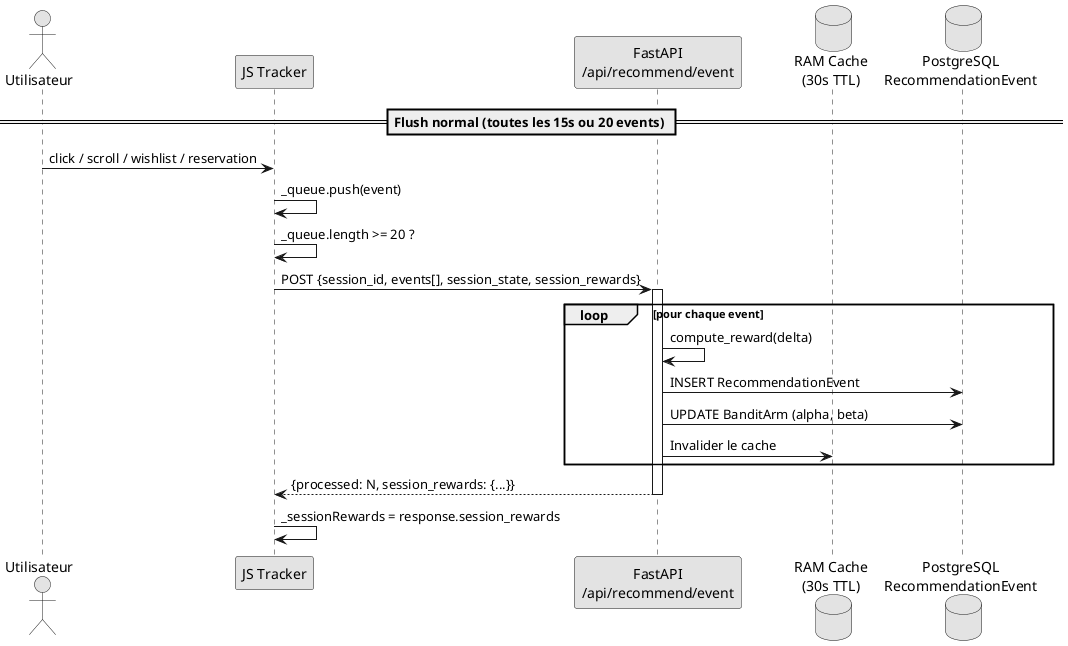
\includegraphics[width=\textwidth]{diagrams/fig_05_tracker_flush.png}
    \caption{Flux de collecte d'événements et mise à jour des matrices LinUCB}
    \label{fig:tracker_flush}
\end{figure}


% ────────────────────────────────────────────────────────────────
\section{Extracteur de tags LLM et jobs nocturnes}
% ────────────────────────────────────────────────────────────────

\subsection{Mise à jour des profils utilisateurs}

Le job \texttt{run\_profile\_update\_job()} s'exécute chaque nuit à 3h00 (fuseau
Africa/Tunis). Il traite uniquement les utilisateurs authentifiés ayant généré des événements de
recommandation dans les dernières 24~heures, rendant le traitement efficace et ciblé. Les
utilisateurs inactifs ne sont pas retraités inutilement.

Pour chaque événement avec récompense positive, les tags de l'annonce sont récupérés.
Pour chaque tag dans cette annonce, l'affinité est mise à jour selon~:
$\text{affinity}[\text{tag}] \mathrel{+}= r \times e^{-\lambda \cdot \Delta t}$ où
$\lambda = \ln(2)/30$ (demi-vie de 30~jours~: un événement de 30~jours contribue à 50\%
d'un événement frais). Après traitement de tous les événements, la composante $x_7$ 
est calculée par transformation exponentielle de l'affinité maximale brute~:
$$x_7 = 1 - e^{-\text{raw\_max}}$$
où $\text{raw\_max} = \max(\text{affinity.values()})$, ce qui reflète 
l'intensité globale d'intérêt de l'utilisateur et reste naturellement 
dans $[0, 1]$ sans normalisation explicite.

Les métriques dérivées sont calculées à partir des événements de réservation uniquement~:
\texttt{avg\_booking\_price} et \texttt{price\_std\_dev} sont extraites des événements de
type \texttt{reservation}~; \texttt{dominant\_trip\_type} est déterminé par le type de voyage
le plus fréquent parmi les 10~dernières réservations. Le profil complet est inséré ou mis à
jour dans la table \texttt{UserProfile} par \texttt{upsert}.


\subsection{Gestion de la dérive conceptuelle}

La dérive conceptuelle dans le contexte des recommandations touristiques se manifeste de
plusieurs façons~: les préférences des utilisateurs évoluent avec les saisons (activités
de plage en été, activités culturelles intérieures en hiver), avec les événements globaux,
et avec la croissance de la plateforme (nouvelles catégories d'annonces). Une matrice LinUCB
entraînée purement sur des données historiques finira par sur-ajuster les anciens patrons.

Le mécanisme de réinitialisation partielle est déclenché tous les 90~jours~ ou plus:
$A_{new} = 0.7 \cdot A + 0.3 \cdot I$ et $b_{new} = 0.7 \cdot b$. Le facteur
$\lambda_{\text{decay}} = 0.7$ oublie progressivement les anciennes données tout en
conservant la structure apprise, et réintroduit de l'incertitude d'exploration en ajoutant
30\% de la matrice identité. Cette approche est plus douce qu'une réinitialisation complète
qui perdrait tout le savoir accumulé.

La vérification de dérive lit l'horodatage de dernière réinitialisation
depuis la table de configuration système, applique la réinitialisation
partielle si 90~jours ou plus se sont écoulés, et sauvegarde les matrices mises à jour.
Le job s'exécute le 1\textsuperscript{er} de chaque mois à 4h00.


\subsection{Planificateur de tâches}

Le planificateur est configuré avec un fuseau horaire fixe, un pool de deux threads de
travail, et une limite d'une instance par job pour empêcher les exécutions chevauchantes.
Quatre jobs sont enregistrés~: la mise à jour des profils (cron quotidien 3h00), la
vérification de dérive (cron mensuel le 1\textsuperscript{er} à 4h00), le rafraîchissement
des tags (cron mensuel le 15 à 2h00), et la persistance des matrices (intervalle de
2~minutes).

Chaque job est encapsulé dans une logique de capture d'erreurs pour qu'une défaillance
isolatrice ne bloque pas les autres jobs. Le planificateur démarre et s'arrête avec le
cycle de vie de l'application, voir le tableau~\ref{tab:scheduler_jobs}.

\begin{table}[H]
    \centering
    \caption{Planning global des tâches automatisées}
    \label{tab:scheduler_jobs}
    \small
    \begin{tabular}{p{3cm} p{1.5cm} p{1.8cm} p{2cm}  p{5cm}}
        \toprule
        \textbf{Job} & \textbf{Type} & \textbf{Heure} & \textbf{Fréquence} &
         \textbf{Impact} \\
        \midrule
        profile\_update & cron & 3:00 & Quotidien & Maj UserProfile actifs \\[2pt]
        concept\_drift & cron & 4:00 & 1\textsuperscript{er}/mois& Reset partiel A,b \\[2pt]
        tag\_refresh & cron & 2:00 & 15/mois & Re-extraction tags \\[2pt]
        matrix\_persist & interval & — & 2 min & Flush RAM$\rightarrow$DB \\
        \bottomrule
    \end{tabular}
\end{table}


% ────────────────────────────────────────────────────────────────
\section*{Conclusion du chapitre}
\addcontentsline{toc}{section}{Conclusion du chapitre}

Ce chapitre a présenté l'implémentation complète du moteur de 
recommandation Hybrid LinUCB du système Guidni. L'ingénierie des 
caractéristiques construit un vecteur de contexte combinant les 
signaux utilisateur et les caractéristiques des annonces. Le moteur 
de scoring équilibre exploitation et exploration avec un mécanisme 
de correction en faveur des annonces sous-exposées. Le tracker 
JavaScript collecte les événements comportementaux en temps réel avec 
une transmission périodique et immédiate pour les signaux de haute 
valeur. Les jobs nocturnes assurent la mise à jour des profils 
utilisateurs, la gestion de la dérive conceptuelle par réinitialisation 
partielle progressive, et le rafraîchissement des tags des annonces.

Le chapitre suivant présentera le déploiement du système et l'architecture de production de la plateforme Guidni, décrivant la topologie d'isolation des conteneurs, la configuration réseau, les spécifications du serveur hôte, l'orchestration Docker Compose et le pipeline de déploiement séquentiel sécurisé.
